%
% Lorentz型の誘電関数のグラフ
%


\documentclass[varwidth=12cm,border=1cm,tikz]{standalone}
% https://latexdraw.com/plot-a-function-and-data-in-latex/
\usepackage[hiragino-pron]{luatexja-preset} % standaloneとlualatexjaを共存させる方法?
\usepackage{tikz}
\usepackage{pgfplots}
\usepackage{physics}

\pgfplotsset{compat = newest}
\pgfplotsset{every axis/.append style={
                    label style={font=\huge},
                    title style={font=\huge},
                    tick label style={font=\huge},
                   }}
 \usepgfplotslibrary{colorbrewer}
 \usetikzlibrary{pgfplots.colorbrewer}
\begin{document}
    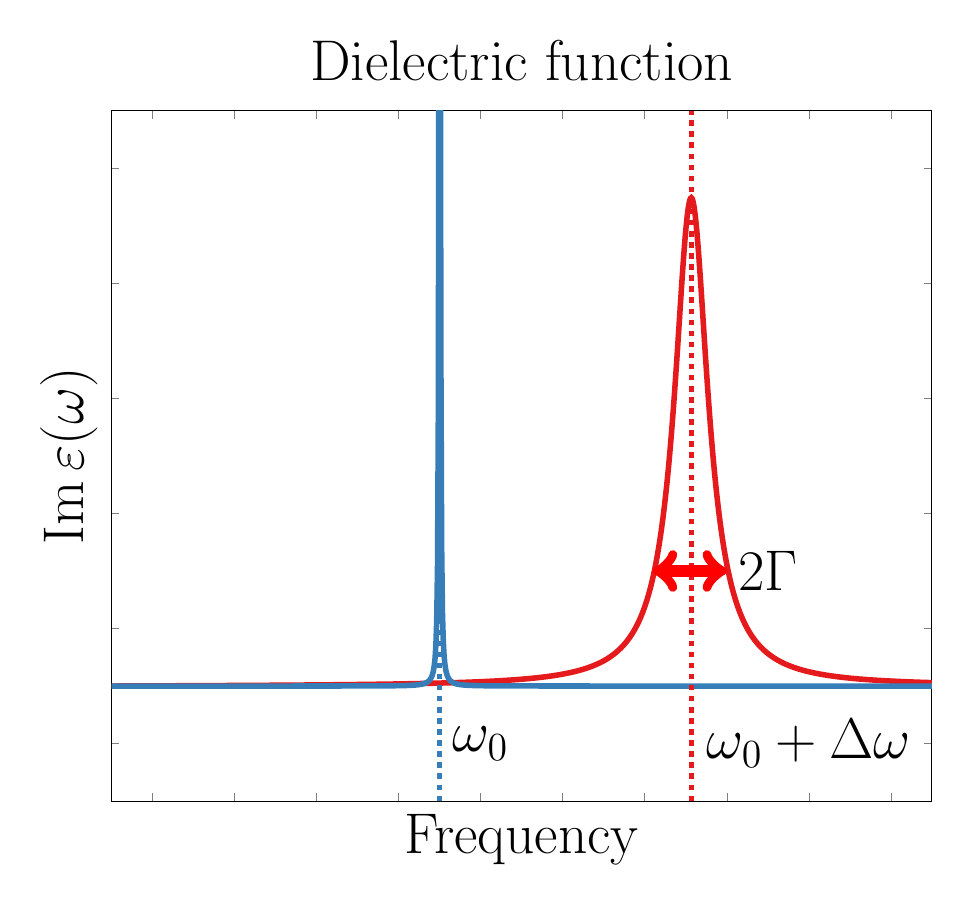
\begin{tikzpicture}
     \tikzset{every node}=[font=\Large]
        % axis環境が2次元plot
        \begin{axis}[ %グラフ設定
            xmin = 0, xmax = 200,
            ymin = -1, ymax = 5,
            ticks=none,
	    xlabel=$\mathrm{Frequency}$,
	    ylabel=$\Im \varepsilon(\omega)$,
	    title=Dielectric function,
            % grid = both,
            minor tick num = 1,
            major grid style = {lightgray},
            minor grid style = {lightgray!25},
            width = 12cm,
%            height = 0.75\textwidth,
            legend cell align = {left},
            legend pos = north west
        ]
            \coordinate (A) at (80,-1); % additional peak @x-axis
	    \coordinate (B) at (80,5);
	 
	 % 誘電関数 虚部
	 \addplot[domain = 0:200,samples=1000,line width=2,Set1-A] {60000*x/((20000-x*x)*(20000-x*x)+100*x*x)};
	 \addplot[domain = 0:200,samples=1000,line width=2,Set1-B] {100*x/((6400-x*x)*(6400-x*x)+0.1*x*x)};

%            \addplot[blue,solid, line width = 2, mark = none] table [x index=2, y index=4] {\au};
%            \addplot[red ,solid, line width = 2, mark = none] table [x index=2, y index=4] {\eu};
	    \addplot[Set1-A, dotted, line width = 2, mark=none] coordinates {(141.4,-1) (141.4,5)}; 
	    \addplot[Set1-B, dotted, line width = 2, mark=none] coordinates {(80,-1) (80,5)}; 
%	    \addplot[blue,dotted, line width = 2, mark=none] coordinates {(598,0) (598,180)};
            %\addplot[red, only marks] table [x ={x}, y = {y2}] {\table};
            %\addplot[teal, only marks, mark = x, mark size = 3pt]
            %    table [x = {x}, y = {y3}] {\table};
	    \node[font=\huge] at (90,-0.5) {$\omega_0$};
	    \node[font=\huge] at (170,-0.5) {$\omega_0+\Delta\omega$};
	    \node[font=\huge] at (160,1) {$2\Gamma$};
	    \addplot[<->,red,line width =4, mark=none]coordinates {(132, 1) (150, 1)};
            \legend{} % no legend
	    %,
            %    Plot only with marks,
            %    Plot with other type of marks}
        \end{axis}
    \end{tikzpicture}
\end{document}

% \documentclass{standalone}

% \usepackage{tikz}
% \usepackage{pgfplots}

% \pgfplotsset{compat = newest}

% \begin{document}
%     \begin{tikzpicture}
%         \begin{axis}[
%             xmin = 0, xmax = 30,
%             ymin = -1.5, ymax = 2.0,
%             xtick distance = 2.5,
%             ytick distance = 0.5,
%             grid = both,
%             minor tick num = 1,
%             major grid style = {lightgray},
%             minor grid style = {lightgray!25},
%             width = \textwidth,
%             height = 0.5\textwidth,
%             xlabel = {$x$},
%             ylabel = {$y$},
%             legend cell align = {left},
%         ]
%             \addplot[
%                 domain = 0:30,
%                 samples = 200,
%                 smooth,
%                 thick,
%                 blue,
%             ] {exp(-x/10)*( cos(deg(x)) + sin(deg(x))/10 )};
            
%             \addplot[
%                 smooth,
%                 thin,
%                 red,
%                 dashed
%             ] file[skip first] {cosine.dat};
            
%             \legend{Plot from expression, Plot from file}
%         \end{axis}
%     \end{tikzpicture}
% \end{document}